%%
%% Author: 伊藤裕貴
%%
\subsection{死んだ電波銀河のシェルからの放射}\label{transients.s3.agn}
電波銀河の主な放射源は、AGNジェットによって形成される電波ローブと呼ばれる広がった構造である。
観測されている電波銀河のサイズは幅広く分布しており、kpc未満のものからMpcを超えるようなものまで存在している。
電波銀河の大きさは、主に年齢 (ジェットの中心核からの噴出が維持されている時間) によって決まり、小さいものは若く、大きいものは年老いていると考えられている。
したがって、小さい電波銀河はいずれ大きい電波銀河に成長するといった描像が広く受け入れられている。

しかしながら、単純に全ての電波銀河が10~kpcを超えるような大きさに成長できるのかはよく分かっていない。
というのも、理論的には 10~kpcに満たない小さくて若い電波銀河 (年齢$10^3$--$10^5$歳の電波銀河) の割合は全体の約 0.01\% と予測されるが、実際の観測では全体の約 10--30\% を占めており、年老いた銀河が予測より少ないためである \citep{Orienti01032010,2010MNRAS.408.2261K}。
この未解決問題について様々なシナリオが提唱されてきているが、一つの自然な解釈は、大多数の電波銀河が若い段階でジェット活動を停止もしくは休止し、成長が止まってしまい「死んでいる」とする解釈である。

このシナリオを検証するためには、死んだ電波銀河を観測でとらえる必要性があるが、ジェットの活動性を失った電波ローブは急激に暗くなってしまうため、従来の観測施設でとらえる事は困難であり、現状は候補天体が数例見つかっている程度である。
さらに最近の理論研究からは、ローブは暗くなるだけではなく放射帯域が10~MHz以下となってしまうため、SKA をもってしても、死んだ天体の電波ローブからの放射を検出する事は難しい事が示されている (Ito et al., 2015, submitted to ApJ)。
しかし電波ローブではなく、それを取り囲む周辺物質から構成される「シェル」は、ジェットの活動が休止した後も急激には減光しないため、SKAによってとらえられる事が期待できる (\Figref{fig:transients.s3.agn.fig1})。
したがって、電波銀河の進化トラック解明への道を切り開くためには、SKAを用いてシェルの観測を行うことが不可欠である。
さらにSKAによって、AGNジェットが周辺環境に与える影響 (AGNフィードバック) や、ジェットが駆動される条件などのサイエンスに関しても迫る事が期待される。
\begin{figure}
		\centering
		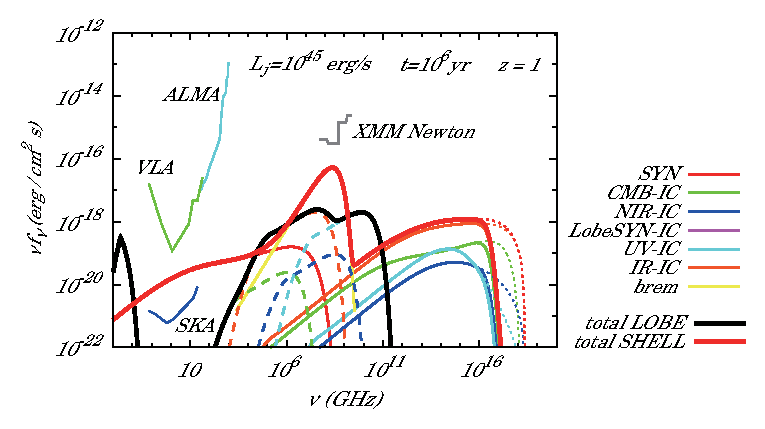
\includegraphics[width=0.8\textwidth]{transients/transients.s3.agn.fig1.eps}
		\caption{ジェットの放出が停止した (死んだ) 電波銀河に付随するローブ (黒実線) 及びシェル (赤実線) のスペクトル。
		電波銀河の年齢を$10^6$年、ジェットが活動を停止するまでの継続時間を$10^5$年と仮定し、また赤方偏移を$z=1$としている (Ito et al., 2015, submitted to ApJ)。}
		\label{fig:transients.s3.agn.fig1}
\end{figure}%
